\chapter{Results}
\label{sec:results}
%In previous chapters, there were introduced different methods available for selected use cases in research in biology and medicine. 
%\section{Virtual Infrastructure}
%\label{sec:resultsinfrastructure}
The pilot virtual infrastructure dedicated for research purposes, as proposed by the author of this thesis (3.), was established to consolidate and share resources among different projects. 
%The paper \cite{kulhanek2010c} \emph{Infrastructure for Data Storage and Computation in Biomedical Research} in Appendix~\ref{app:infrastructure} describes result of establishing the virtualization on physical infrastructure to share computational power among different platforms.
\section{Medical Image Sharing}
\label{sec:resultsimages}

The pilot infrastructure of several servers was installed in several institutions in Prague, Czech Republic. Globus Toolkit and Globus MEDICUS were installed on them,
the system connected with MEDIMED project integrates classical production system to share medical images with grid-based PACS system via the DICOM protocol. The grid-based system was tested with about 1300 DICOM records and enhanced with simple DICOMViewer available as web application. 
The grid-based solution allows to store large set of data records and manage replicas. The standard protocol to transfer data files gridFTP allows to effectively transfer parts of the files to the desired location from existing replicas within grid infrastructure to a desired location where an image processing can be performed. Current systems of sharing medical images may suffer from the problem of single point of failure or bottleneck. The grid-based solution brings robustness against the mentioned problems. 

\section{Remote Voice Analysis}
\label{sec:resultsvoice}

RDP protocol was customized and support for transferring sound recording was implemented. A client plugins were customized for the Linux "rdesktop" application as well as for the Windows default "tsclient" application. The plugin initiates sound recording from a sound device and creates a custom RDP channel. A raw data obtained from the sound device is transferred to the custom RDP channel. The server plugin writes the data from the custom channel directly to a file in WAV format and offers sound samples to the analytical application for real-time processing. The schematic architecture of the system is in Figure \ref{fig:architecturesound}.

\begin{figure}[hbt]
    \centering
     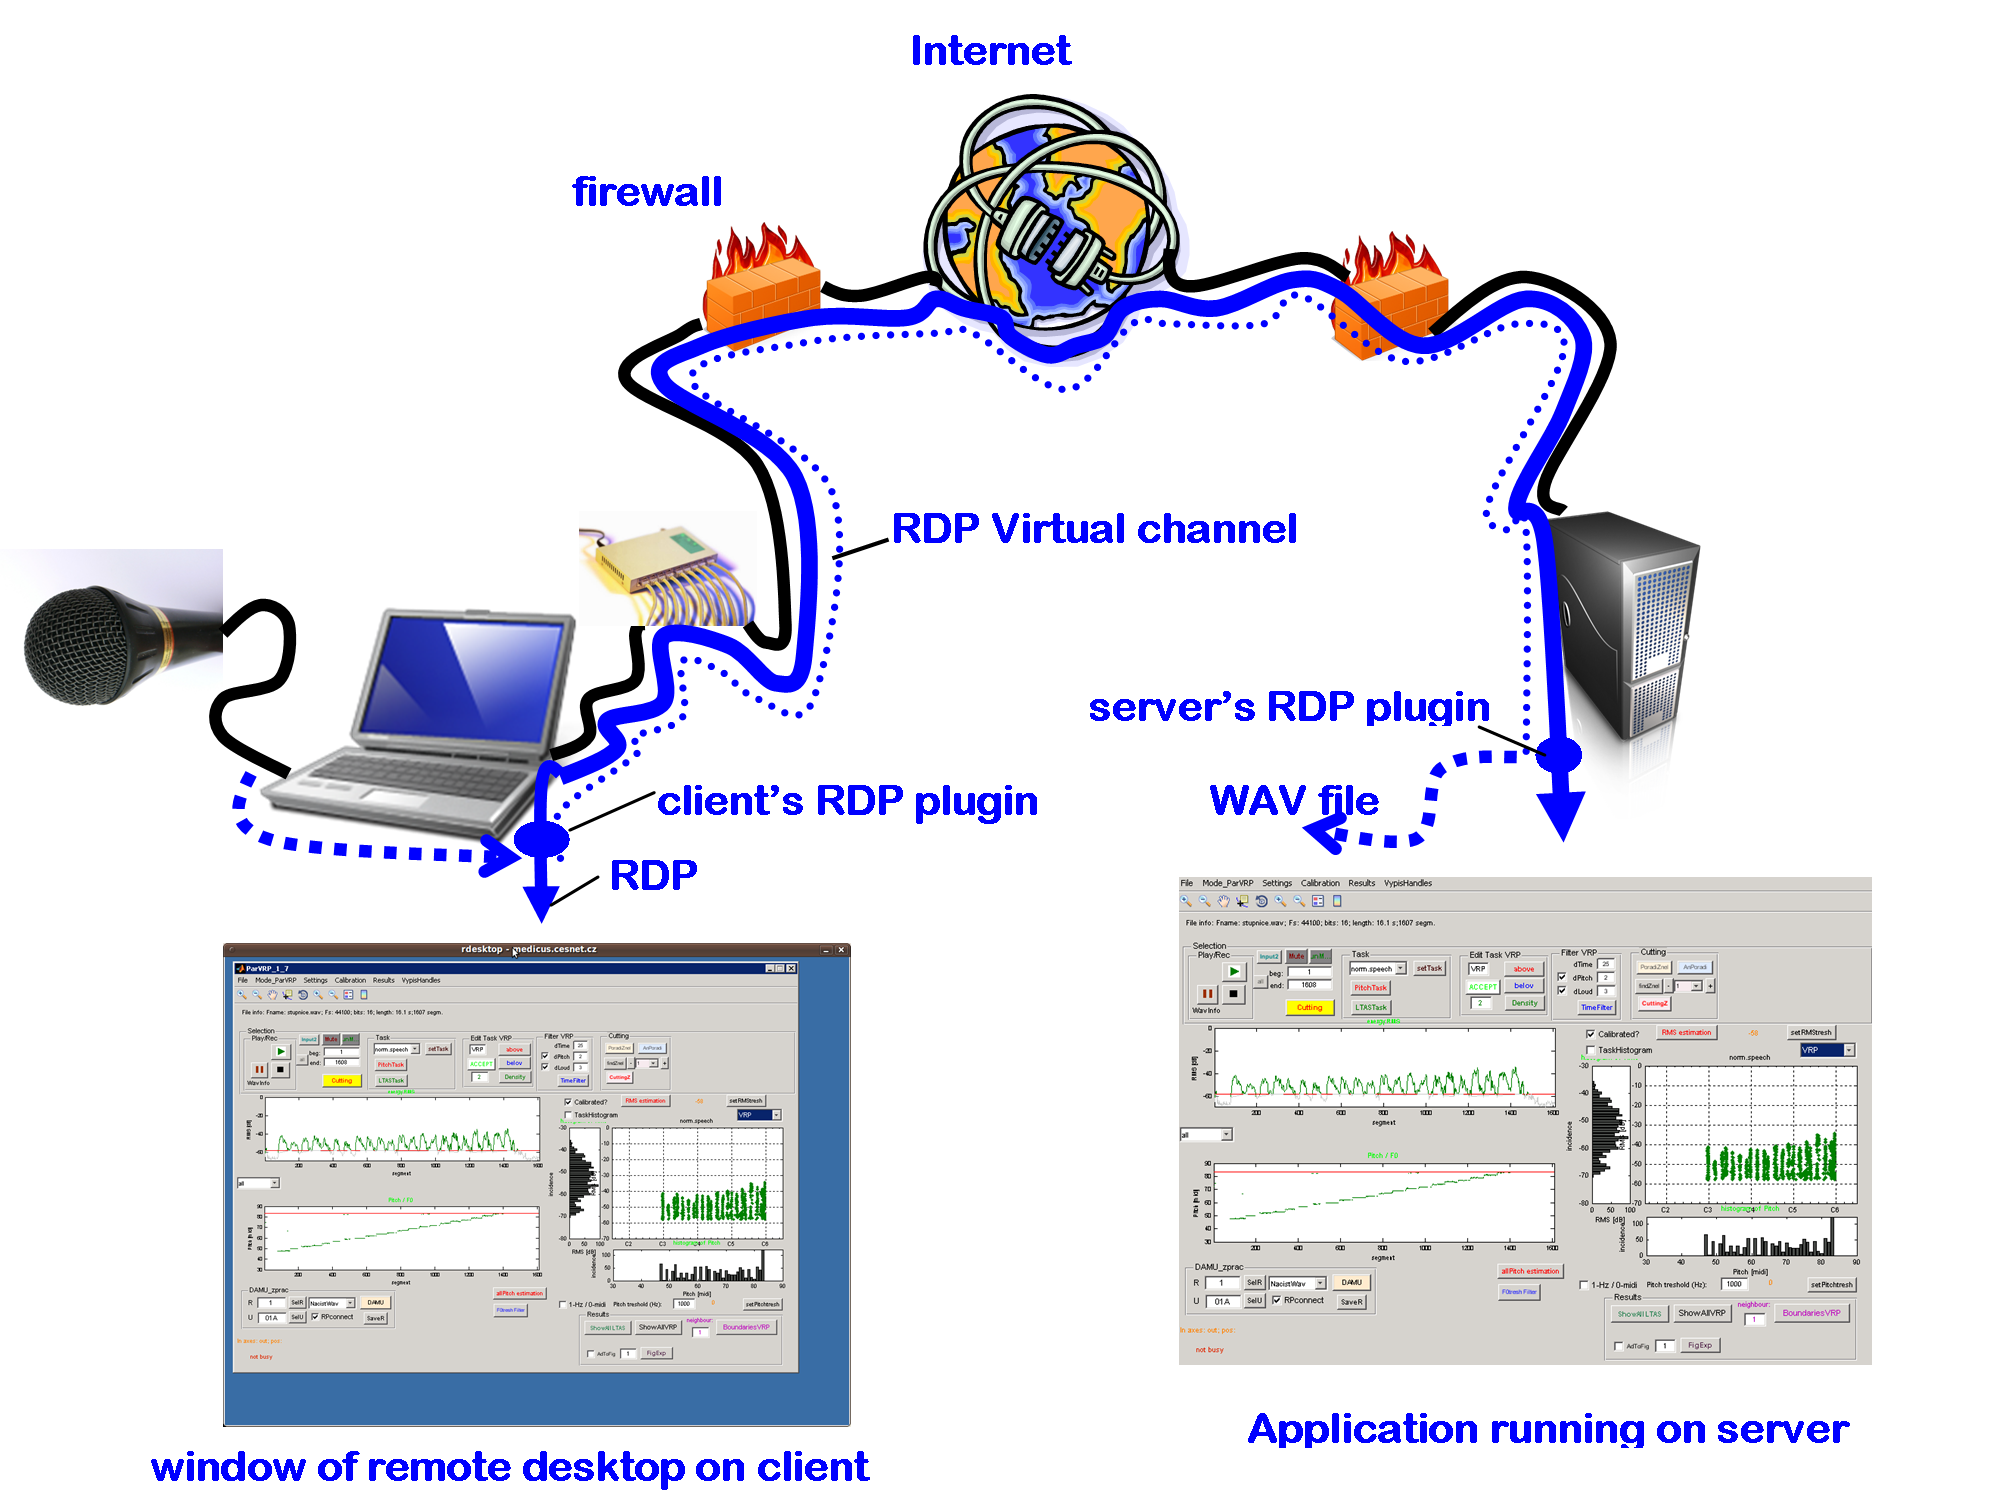
\includegraphics[width=0.75\textwidth]{schemasystemu.png}  
    \caption{Architecture of a system for remote voice analysis and RDP plugins for sound recording redirection.}
    \label{fig:architecturesound}
\end{figure}

The default sound recording features of RDP protocol version 5.2 and 7.0 degrades sound quality transferred to the server application, furthermore, some samples of the sound were lost and sound become garbled or scratchy. The sound quality using the custom RDP channel is without loss of information and acceptable for further analysis. Additionally, the remote application with custom RDP plugin was packaged as a virtual machine template and can be provisioned on cloud computing infrastructure in case of the need.

The application allows to record the voice of patient, the voice signal is transferred to remote application where it is processed and analyzed, the results are visualized in real-time. The application is now used by several voice therapists and voice pedagogues in different areas of the Czech Republic and Slovakia to analyze the voice in non-invasive way in order to see e.g. the progress of the voice training methods.

\section{Computational Physiology}
\label{sec:resultsestimation}

\subsection{Modeling Methodology}

Within the thesis, the modeling methodology was improved in an area of modeling cardiovascular system in a complex integrative way, which can be used for research and educational purposes. A set of recommendation was published: (1) to use acausal connector (special purpose class where no causality (what is input and output) is defined), (2) utilize object-oriented features in order to separate pure model from the specific experiment, (3) combine textual and diagram notation in order to express mathematical equations/component relations.
%The modeling tool will decide the direction of computation (what will be input and output) upon compilation time. 
This lead to more exact and understandable model for domain experts. 
The table \ref{table:physiolibrary} contains definition of basic components of hydraulic domain used to model cardiovascular system. Figure \ref{fig:fernandezmodel} shows an  implementation of the model published originally by Fernandez de Canete \cite{FernandezDeCanete2013} in Modelica language published in (7.). Such medium complex models are important for further studies. Methodology and it's usage in education is described in publication by the author of this thesis in (1.) and (7.).


\begin{figure}[ht]
    \centering
    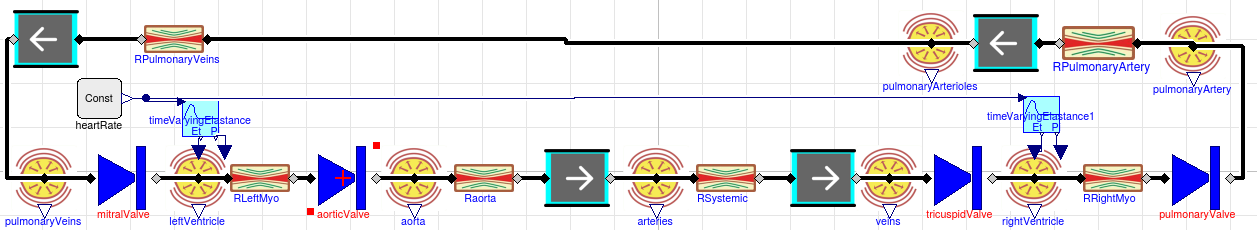
\includegraphics[width=1\textwidth]{fernandezmodel.png}
    \caption{Implementation of the model of cardiovascular system \cite{FernandezDeCanete2013} in Modelica language using components of Physiolibrary (21.). The connected components is compiled by the Modelica tool with the equation defined in Table \ref{table:physiolibrary}. In this case the 209 equations (133 are trivial and 76 are non-trivial equations) are generated and causality is solved by the tool.
    }
    \label{fig:fernandezmodel}
\end{figure}

%A set recommendation regarding causal and acausal approach in using Modelica for modeling pulsatile cardiovascular system (CVS)\nomenclature{CVS}{Cardiovascular System} was published in (1.) and implementation of cardiovascular system controlled by the baroreceptor control system was implemented showing robust solution.

\subsection{Parameter Estimation}

The proposed architecture of the system for parameter estimation (Figure  \ref{fig:architectureestimation}) was influenced by the need of some interactivity and for the overall accessibility for users, which is fulfilled by the web UI. 

\begin{figure}[hbt]
    \centering
     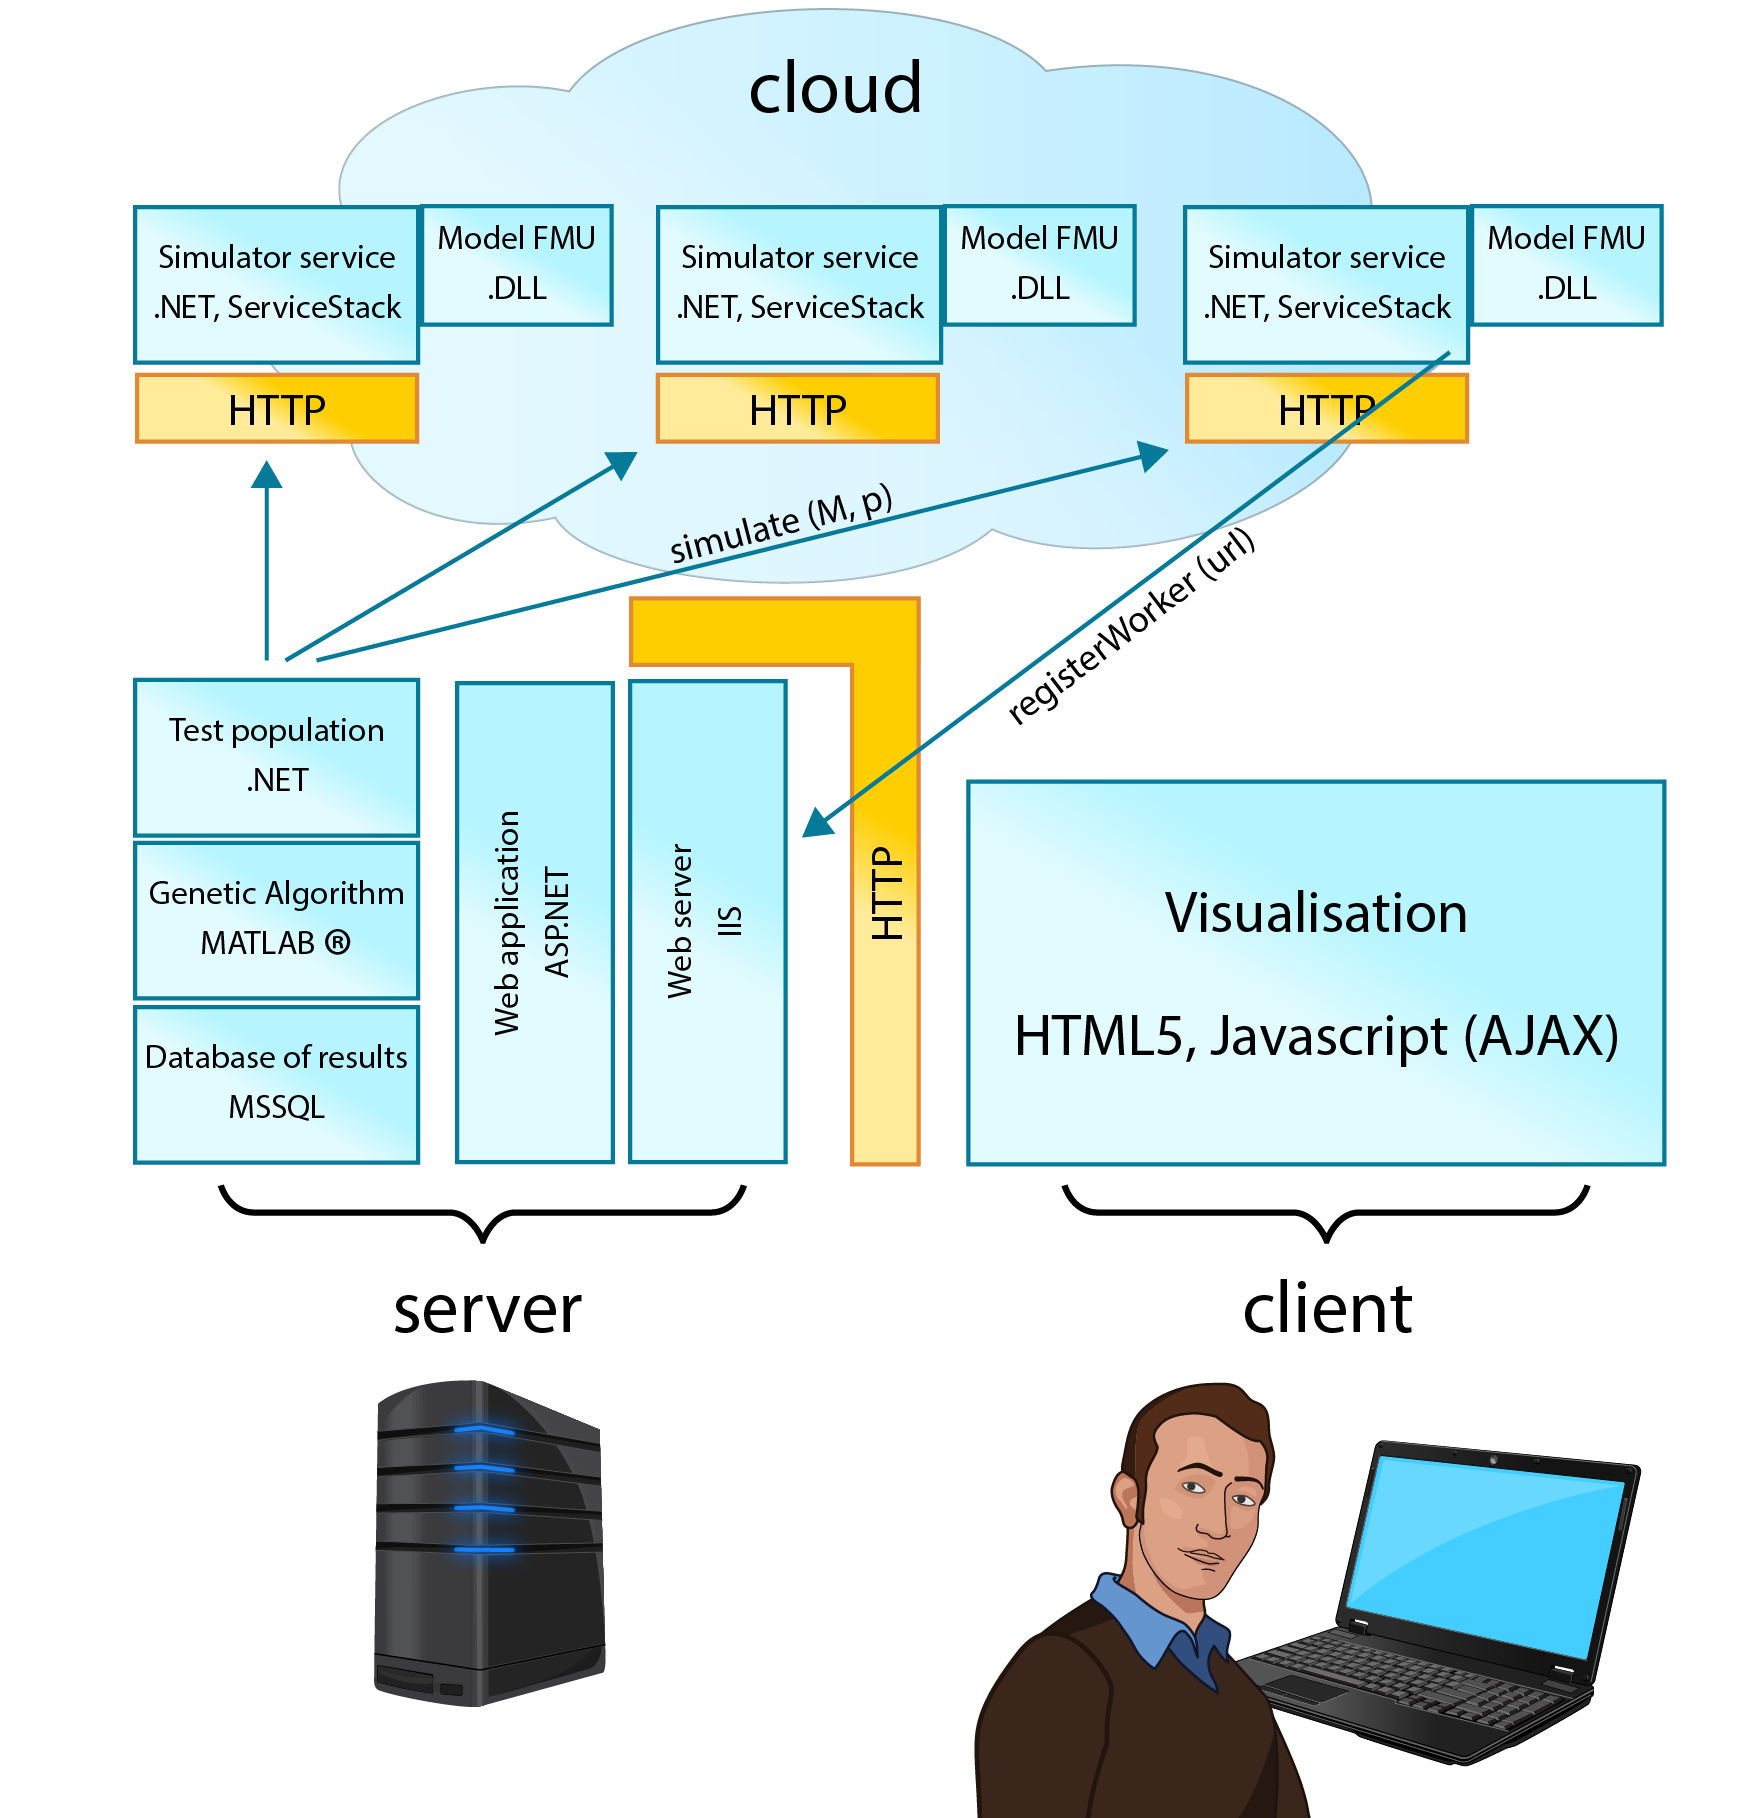
\includegraphics[width=0.75\textwidth]{../img/chapter3-architekturaestimation-01.png}  
    \caption{Architecture of a system that employs genetic algorithm and distributes the task \emph{simulate} into a cloud computing environment.}
    \label{fig:architectureestimation}
\end{figure}

The Modelica models is exported to standardized FMU and wrapped with a RESTful webservice implemented in .NET ServiceStack framework\footnote{\url{https://servicestack.net} accessed April 2015} allowing remote control of simulation. In the time of writing this thesis, the most stable Modelica tool was Dymola version 2015\footnote{\url{http://www.dynasim.se} - Dymola tool, accessed March 2015}, and most stable export was to FMU for a MS Windows platform. Several RESTful web services packaged in a virtual machine template was instantiated in scientific cloud.
The overall performance and speedup estimation were tested against the Modelica implementation of complex physiological model HumMod \cite{Kofranek2011hummod}, the Modelica implementation of a model of hemodynamics of the cardiovascular system, originally published by Meurs \cite{Meurs2011} and the model of $O_2$, $CO_2$ and $H^+$ binding on hemoglobin, published by Matejak et al. and contributed by the author of this thesis (2.)%\cite{Matejak2014sj} 

\sisetup{round-mode=figures,round-precision = 3}
\begin{table}[htb]
\footnotesize
\begin{tabular}{|l|r|r|r|r|r|r|r|r|r|}
\hline
compl. & name & S(10) & S(20) & S(30) & S(40) & S(50) & S(60) & S(80)& S(160)\\
\hline
high & HumMod \cite{Kofranek2011hummod} & $\num{10}$ & $\num{20.4}$ & $\num{24.8}$ & $\num{35.4}$ & $\num{41.8}$ & $\num{49.83}$ & $\num{63.9807249802}$ & $\num{121.5389821285}$ \\
medium & Meurs2011\cite{Meurs2011} & $\num{8.7}$ & $\num{16.6}$ & $\num{24.4}$ & $\num{29.6}$ & $\num{32.9}$ & $\num{38.65}$ & $\num{55.9311360464}$ & $\num{53.0128125}$ \\
low & Matejak2014\cite{Matejak2014sj} & $\num{7.5}$ & $\num{11.8}$ & $\num{12.5}$ & $\num{15.4}$ & $\num{15.7}$ & $\num{14.73}$ & $\num{16.6865881526}$ & $\num{12.5500720509}$\\ \hline
\end{tabular}
\caption{Comparison of model scalability and complexity. Speedup $S$ on 10 CPUs till 160 CPUs of parameter estimation, using cloud computing cluster on 1-6 virtual machines, each 10 CPUs (2x5-core Intel E5-2620 2GHz, 1Gbit/s Ethernet.) (resp. 5-10 virtual machines, each 16 CPUs on physical hardware 2x 8-core Intel E5-2670 2.6GHz). Genetic algorithm configured with a population $120$ (resp. $640$) individuals for $10$ (resp. $20$) generations. Speedup estimated from measuring the serial computation on 1 CPU.}
\label{table:speedupresult3}
\end{table}

To summarize the results from Table \ref{table:speedupresult3}, the low complex model scales up to 40 CPUs with a speedup of 15. The medium complex model scales up to 80 CPUs with a speedup of 56 and complex model scales up to 160 CPUs (and probably more) with a speedup of 122. Practically, good parameter estimation was obtained after 200 generations with population of 640, which implicates that the computation time can be reduced from four days to 47 minutes in the case of complex model and from 14 hours to 15 minutes in the case of medium complex model.

The parameter estimation on low complex model suffers with major network overhead. Thus, such low complex models can be effectively identified on local cluster with comparable time of computation.

\section{Adair-based Oxygen Binding to Hemoglobin}
The parameter estimation was used to compute parameters of newly constructed model of hemoglobin integrating $O_2$ , $CO_2$ and $H^+$ binding based on theoretical principles, which were verified on the parameter estimation algorithm system described above and noted as the low complex model Matejak2014 published as (2.).
The author of this thesis implemented the model in Modelica language and estimated parameters of dissociation constants of the chemical reaction of oxygen binding to different forms of hemoglobin comparing the simulated saturation curves of $O_2$ with the experiments published in scientific literature.

\section{Parameter Sweep}
The desktop grid BOINC framework was customized and a system was established for parameter sweep application. The established project, \emph{Physiome@home}, and it's project web page, \url{http://physiome.lf1.cuni.cz/ident3/physiome}, manages workunit tasks which are downloaded and executed by BOINC workers. The worker application consist of a packaged model that is exported as FMU for a Windows platform and of a universal preconfigured wrapper application provided by BOINC framework, which integrates generic application with a BOINC manager on the desired volunteer computer. Workunits are generated by a tool within BOINC framework.

Parameter sweep method can enhance the ability to perform identifiability and uncertainity analysis of general complex models and can deliver results of explored parameter space in a reasonable time.

%\section{Parameter Sweep}
%\label{sec:resultsboinc}

